\documentclass[twocolumn]{iopjournal}

\usepackage{amsmath,amssymb,amsfonts}
\usepackage{amsthm}

\fancyhfoffset[L]{0mm}
\setlength{\marginparwidth}{0pt}
\setlength{\marginparsep}{0pt}

% ==========================================
% ZENODO PREPRINT HEADERS (ACTIVE)
% ==========================================
\renewcommand{\articletype}[1]{%
  {\vspace*{-8mm}\noindent \Large \sf Preprint}\par
  \vspace*{6mm}\noindent{\scriptsize \sf{\bfseries \MakeUppercase{#1}}}}

\fancyhead[L]{}
\fancyhead[R]{}

\hypersetup{pdftitle={Vortices of the Stellated Octahedron}, pdfauthor={Stephen Nelson}, pdfsubject={Gravity Field Dynamics (GFD)}, pdfkeywords={stellated octahedron, vortex, standing wave, tetrahedral symmetry, Field Origin, proof}}

\newtheorem{lemma}{Lemma}
\newtheorem{theorem}{Theorem}
\newtheorem{proposition}{Proposition}
\newtheorem{corollary}{Corollary}
\theoremstyle{definition}
\newtheorem{definition}{Definition}
\theoremstyle{remark}
\newtheorem*{remark}{Remark}

\begin{document}

\articletype{Proof}

\title{Vortices of the Stellated Octahedron}

\author{Stephen Nelson}

\affil{Field Dynamics Research}

\ead{stephen@fielddynamics.org}

\begin{abstract}
Gravity Field Dynamics works with a cube holding a stellated
octahedron: two tetrahedra, TetA and TetB, whose overlap, the central
octahedron, is the Field Origin. We study real symmetric Hamiltonians
with the tetrahedral symmetry $T_d$ on two graphs built from the cube,
with TetA and TetB free to differ: one on its points (the corners, and
the Field Origin's octahedron and centre), and one on its faces (the
Triforce sub-channels and the centre). We prove that they carry vortices: stationary states
that wind about an axis and carry a circulating current around an
axis on which they vanish. On the cube's points, about each axis of the
Field Origin's octahedron,
there are exactly three vortices and three antivortices, with distinct
energies interlacing the corner energies, outside an explicit
exceptional set. Their current through any half-plane bounded by the
axis is $I = (E - \Delta_f - 2h)\lvert\rho\rvert^2$, where $\rho$ is
the amplitude on each vertex of the Field Origin's equatorial ring and
$h$ the hopping along the octahedron's edges, and the corners are
locked to that ring: the circulation runs through the Field Origin
around its empty centre. Read as modes of a network of coupled
oscillators, each vortex is a rotating wave, and a vortex plus its
antivortex is a standing wave. On the Triforce faces the winding space
about a leg splits as $W \oplus W'$ by representation theory. On $W$
every energy is doubled, with the two energies in closed form; on $W'$
there are generically six vortices, each turning a star point's outer
sub-channel around the leg, whose empty core is the gravitational
coupling line through the Field Origin. Hand proofs are given throughout;
the all-parameter statements are also checked symbolically, and the
generic statements are certified exactly over $\mathbb Q(i)$ and
$\mathbb Q(\omega)$ in code that uses no computer algebra.
\end{abstract}

\keywords{stellated octahedron, vortex, ring current, standing wave,
tetrahedral symmetry, Field Origin, Triforce, proof}

% ======================================================================

\section*{Setting}

\textbf{The cube graph $\mathcal C$} ($1 + 6 + 8 = 15$ sites, the cube's
points): the Field Origin, the
central octahedron in which the chambers intersect~\cite{NelsonColes},
given by its centre $O$ and its six vertices at the cube's face centres
$\pm\hat x,\pm\hat y,\pm\hat z$; and the eight corners $(\pm1,\pm1,\pm1)$,
with TetA the four with $xyz = +1$ and TetB the four with
$xyz = -1$~\cite{NelsonGram,Coxeter1973}. Bonds: $O$ to every other
site; each octahedron vertex to the four corners of its face; and the
twelve edges of the octahedron.

\textbf{The Triforce graph $\mathcal T$} ($1 + 8 + 24 = 33$ sites, the
cube's faces): $O$; the eight central
tiles, the medial triangles of the eight tetrahedron faces (these are
the octahedron's faces); the 24 outer tiles, three per face, which
are the exposed faces of the eight star points. Bonds: two tiles
sharing an edge, and each central tile to $O$. A tile's position is
its centroid. In the archive's terms~\cite{NelsonTriforce} each face is
a triforce of 3 outer sub-channels and 1 central sub-channel: a star
point's three outer tiles form the outer sub-channel at that vertex,
shared by its three faces (spatial coupling), and a central tile couples
through the Field Origin to its partner face, along the line penetrator
$\to$ centroid $\to O \to$ partner centroid $\to$ partner penetrator
(gravitational coupling).

\textbf{The bond sets.} These graphs are not nearest-neighbour graphs of
the point set: $\mathcal C$ contains the $O$--corner bonds (length
$\sqrt3$) and leaves out the cube's twelve edges (length 2, each joining
a TetA corner to a TetB corner). In both graphs TetA and TetB are
coupled only through the Field Origin, its octahedron and its centre,
which is GFD's position that TetB is reached only through the Field
Origin~\cite{NelsonColes}; by symmetry alone the cube's edges would also
be allowed~\cite{NelsonCoupling}. Every result below is a result about
these graphs. The remark \emph{Other bonds} (Section~5) records what changes with the cube's edges.

\textbf{Hamiltonians.} $H$ is real symmetric, supported on the diagonal
and the bonds, and invariant under $T_d$ (24 elements, the symmetries
that keep TetA and TetB). We write site energies on the diagonal and
$H_{ij} = -t_{ij}$ on bonds. $H$ has one free real parameter per
$T_d$-orbit of sites and of bonds: 10 for $\mathcal C$ and 15 for
$\mathcal T$. The statements below hold for this class, under the
hypotheses stated with each.

\textbf{Axes.} In $\mathcal C$ the axis is an octahedron axis $\hat z$,
with symmetry the rotoreflection $S:(x,y,z)\mapsto(-y,x,-z)$, of order
4. In $\mathcal T$ it is a leg $\hat n = (1,1,1)/\sqrt3$, with symmetry
the rotation $C:(x,y,z)\mapsto(z,x,y)$, of order 3. Both lie in $T_d$.
The symmetry acts on states by $(S\psi)_{\sigma(i)} = \psi_i$, with
$\sigma$ the induced permutation of sites.

\textbf{Half-planes.} Bonds are straight segments. A half-plane $\Pi$
bounded by the axis is taken in general position: no site off the axis
lies on it. In both graphs no bond joining two off-axis sites meets the
axis (checked), so each such bond sweeps an angle less than $\pi$ about
the axis and crosses $\Pi$ at most once.

\begin{definition}
A \emph{winding state} satisfies $S\psi = \lambda\psi$ (or
$C\psi = \lambda\psi$) with $\lambda$ a primitive root of unity:
$\lambda = \pm i$ for $S$, $\lambda = \omega^{\pm1}$ for $C$. Under
$i\dot\psi = H\psi$, the \emph{bond current} from $i$ to $j$ is
$J_{i\to j} = 2\,\mathrm{Im}(\bar\psi_jH_{ji}\psi_i) = -J_{j\to i}$.
The \emph{circulating current} $I(\psi)$ of a stationary state,
$H\psi = E\psi$, is the total current through a half-plane bounded by
the axis, counted in the right-handed sense about the axis. A
\emph{vortex} is a stationary winding state with $I(\psi) \neq 0$; its
complex conjugate is its \emph{antivortex}.
\end{definition}

% ======================================================================

\section{General lemmas}

\begin{lemma}[Conservation]
$d\lvert\psi_j\rvert^2/dt = \sum_i J_{i\to j}$. Hence for a stationary
state the net current into every site is zero.
\end{lemma}

\begin{proof}
$d\lvert\psi_j\rvert^2/dt = 2\,\mathrm{Re}(\bar\psi_j\dot\psi_j)
= 2\,\mathrm{Im}(\bar\psi_j(H\psi)_j)$, and the diagonal term
$2\,\mathrm{Im}(H_{jj}\lvert\psi_j\rvert^2)$ vanishes. For
$\psi(t) = e^{-iEt}\psi$ the density is constant.
\end{proof}

\begin{lemma}[Empty axis; well-defined current]
\label{lem:axis}
Every winding state vanishes at every site on the axis. For a
stationary winding state, $I(\psi)$ is the same for every half-plane
bounded by the axis.
\end{lemma}

\begin{proof}
A site on the axis lies in an orbit of the symmetry of length $\ell$
smaller than its order ($O$ is fixed; in $\mathcal C$ the axial
vertices $\pm\hat z$ form an orbit of length 2). There
$\psi = \lambda^\ell\psi$ with $\lambda^\ell \neq 1$, so $\psi = 0$,
and bonds at axis sites carry no current. Sum Lemma~1 over the sites
in the wedge between two half-planes: bonds inside the wedge cancel,
each remaining bond crosses one boundary once, and none passes through
the axis. So the two half-planes carry the same current.
\end{proof}

\begin{lemma}[Antivortices]
If $\psi$ is a stationary winding state with eigenvalue $\lambda$, then
$\bar\psi$ is one with eigenvalue $\bar\lambda$, at the same energy, and
$I(\bar\psi) = -I(\psi)$.
\end{lemma}

\begin{proof}
$H$ is real and the symmetry is a real permutation; and
$J_{i\to j}(\bar\psi) = -J_{i\to j}(\psi)$.
\end{proof}

\begin{lemma}[Existence]
$H$ preserves the winding space $V_\lambda$, which has an orthogonal
basis $v_k$ with $v_k[\sigma^jx_k] = \lambda^{-j}$, one vector per orbit
of full length. So $V_\lambda$ has an orthonormal basis of stationary
winding states. $\dim V_{\pm i} = 3$ in $\mathcal C$, and
$\dim V_{\omega^{\pm1}} = 10$ in $\mathcal T$.
\end{lemma}

\begin{proof}
$H$ commutes with the symmetry; the $v_k$ are eigenvectors with
eigenvalue $\lambda$ and have disjoint supports. The orbits of full
length number $(15-3)/4 = 3$ and $(33-3)/3 = 10$.
\end{proof}

\begin{remark}[Time reversal]
By Lemma~3 every vortex level is at least doubly degenerate, shared
with its antivortex. Within such a level the vortex, the antivortex
and the real combination of Proposition~1(ii) are equally good
eigenstates, and any time-reversal-invariant mixed state (thermal,
say) carries no net current. The theorems show which current-carrying
states exist; a particular vortex is selected only by an initial
condition or by breaking time reversal (a flux, a rotation). These are
the discrete analogues of the degenerate $m = \pm1$ orbitals behind
the ring currents of aromatic molecules~\cite{London1937,Pople1956,
SteinerFowler2001}, and they are not persistent currents in the
equilibrium sense of~\cite{BIL1983}.
\end{remark}

% ======================================================================

\section{The cube's points}

Take $\lambda = +i$. In the normalised basis (equatorial ring
$\pm\hat x,\pm\hat y$; TetA corners; TetB corners) of $V_{+i}$, every
$H$ in the class acts as
\begin{equation}
H_+ = \begin{pmatrix}\Delta_f & a & b\\ \bar a & \epsilon_A & 0\\
\bar b & 0 & \epsilon_B\end{pmatrix},\quad
\lvert a\rvert^2 = 2c_A^2,\ \lvert b\rvert^2 = 2c_B^2,
\label{eq:block}
\end{equation}
with $\Delta_f$ the octahedron-vertex energy, $\epsilon_{A,B}$ the
corner energies, and $c_{A,B}$ the vertex-to-corner hoppings. Indeed
the ring vertex $\hat x$ meets the TetA corners $(1,-1,-1)$ and
$(1,1,1) = \sigma(1,-1,-1)$, consecutive in their orbit, so
$\lvert a\rvert = c_A\lvert 1 + \lambda\rvert = \sqrt2\,c_A$, and
likewise for $b$. The octahedron edges add $-h(\lambda + \bar\lambda) =
0$ on the ring and couple it otherwise only to $\pm\hat z$, where
winding states vanish; the energy and hoppings of the Field Origin's
centre $O$ drop out for the same reason. No bond joins a TetA corner to a TetB corner.

\begin{theorem}[Vortices of the cube]
\label{thm:cube}
Let $c_Ac_B \neq 0$ and $\epsilon_A \neq \epsilon_B$. Then:
\begin{enumerate}
\item[(i)] up to scale there are exactly three stationary winding
  states with $\lambda = +i$, one at each root of
  \begin{equation}
  E - \Delta_f = \frac{2c_A^2}{E - \epsilon_A} + \frac{2c_B^2}{E - \epsilon_B},
  \label{eq:secular}
  \end{equation}
  with one root in each of the three intervals cut by $\epsilon_A$ and
  $\epsilon_B$; and three antivortices at the same energies;
\item[(ii)] each has amplitude of modulus $\lvert\rho\rvert \neq 0$ on
  every vertex of the octahedron's ring, and the corners are locked to
  it: with $\rho, p, q$ the amplitudes on $\hat x$, on a TetA corner and
  on a TetB corner (up to the winding phase),
  $p = \bar a\rho/(E - \epsilon_A)$, $q = \bar b\rho/(E - \epsilon_B)$;
\item[(iii)] its circulating current is
  \begin{equation}
  I = (E - \Delta_f - 2h)\,\lvert\rho\rvert^2 ;
  \label{eq:current}
  \end{equation}
\item[(iv)] it is a vortex unless $E = \Delta_f + 2h$, which requires
  $\Delta_f + 2h$ to solve (\ref{eq:secular}); at $h = 0$ this is
  $c_A^2(\Delta_f - \epsilon_B) + c_B^2(\Delta_f - \epsilon_A) = 0$.
\end{enumerate}
At $\epsilon_A = \epsilon_B$ one of the three has $\rho = 0$ and
$I = 0$.
\end{theorem}

\begin{proof}
The rows of $H_+w = Ew$, with $w = (\rho, p, q)$ (site amplitudes,
proportional to the basis coordinates), give
$a p + b q = (E - \Delta_f)\rho$, $\bar a\rho = (E - \epsilon_A)p$ and
$\bar b\rho = (E - \epsilon_B)q$. Now $\det(H_+ - E)$ is
$2c_A^2(\epsilon_A - \epsilon_B)$ at $E = \epsilon_A$ and
$2c_B^2(\epsilon_B - \epsilon_A)$ at $E = \epsilon_B$, both nonzero, so
no root equals $\epsilon_{A,B}$, and $\rho = 0$ would force
$p = q = 0$. Eliminating $p, q$ gives (\ref{eq:secular}). The function
$F(E) = E - \Delta_f - 2c_A^2/(E-\epsilon_A) - 2c_B^2/(E-\epsilon_B)$
has $F' = 1 + 2c_A^2/(E-\epsilon_A)^2 + 2c_B^2/(E-\epsilon_B)^2 > 0$,
runs from $-\infty$ to $+\infty$ on each of the three intervals, and
so has exactly one root in each. For (iii), a half-plane crosses one
edge of the ring, from $\hat x$ to $\sigma(\hat x) = \hat y$ in the
positive sense, carrying
$2\,\mathrm{Im}(\overline{\lambda^{-1}\rho}\,(-h)\,\rho) = -2h\lvert\rho\rvert^2$,
and vertex--corner bonds, whose sum, by the row equations and
(\ref{eq:secular}), is $(E - \Delta_f)\lvert\rho\rvert^2$ (verified
symbolically for three half-planes; Lemma~\ref{lem:axis} makes it
independent of the half-plane). At $\epsilon_A = \epsilon_B$,
$E = \epsilon_A$ is a root of $\det(H_+ - E)$ with $\rho = 0$.
\end{proof}

\begin{corollary}[Without the Field Origin's octahedron]
Remove the octahedron, keeping the Field Origin's centre $O$ and the
corners, with the bonds of $\mathcal C$. Winding states exist ($\dim V_{+i} = 2$), but they
vanish at $O$ and every remaining bond touches $O$, so $I = 0$: there
are no vortices.
\end{corollary}

The corollary depends on the bond set, and so on GFD's position that
TetB is reached only through the Field Origin. With the cube's edges
added, the corners circulate on their own: at $\epsilon_A = 0$,
$\epsilon_B = 1$ and cube hopping 1, the two winding eigenstates carry
currents $\pm1/\sqrt5$ (normalised, exact).

\begin{proposition}[Rotating and standing waves]
\label{prop:standing}
Read a vortex $\psi$ at energy $E > 0$ as the complex amplitude of a
real field $u(t) = \mathrm{Re}(e^{-iEt}\psi)$, a mode of frequency $E$
of a network of coupled oscillators ($J_{i\to j}$ is then the rate at
which amplitude moves along the bond). Then:
\begin{enumerate}
\item[(i)] $Su(t) = u(t - \tfrac{\pi}{2E})$: a quarter turn of the
  pattern (with the top--bottom flip) equals a fixed delay, so the
  pattern rotates about the axis, once per period;
\item[(ii)] $\phi = \psi + \bar\psi$ is real and stationary at the same
  energy, carries no current on any bond, and its field
  $\cos(Et)\,\phi$ oscillates in place: vortex and antivortex together
  make a standing wave.
\end{enumerate}
In the quantum reading $\psi(t) = e^{-iEt}\psi$, by contrast,
$S\psi(t) = i\psi(t)$: the quarter turn is a global phase, and the
density and every bond current are constant in time.
\end{proposition}

\begin{proof}
(i) $Su(t) = \mathrm{Re}(e^{-iEt}\,i\psi) = \mathrm{Re}(e^{-iE(t-\tau)}
\psi)$ for $E\tau = \pi/2$. (ii) uses Lemma~3: $\bar\psi$ is
stationary at $E$; a real vector has
$\mathrm{Im}(\phi_jH_{ji}\phi_i) = 0$; and
$\mathrm{Re}(e^{-iEt}\phi) = \cos(Et)\phi$.
\end{proof}

% ======================================================================

\section{The Triforce faces}

\begin{theorem}[Vortices of the Triforce faces]
\label{thm:triforce}
In $\mathcal T$, with $\lambda = \omega$ about a leg:
\begin{enumerate}
\item[(i)] $V_\omega$ has dimension 10, and every vector in it vanishes
  on the leg: at $O$ and at the two central tiles it passes through;
\item[(ii)] $V_\omega = W\oplus W'$, an orthogonal sum preserved by every
  $H$ in the class, with $W = V_\omega \cap (E \oplus T_1)$ ($\dim 4$,
  supported on the outer tiles) and $W' = V_\omega \cap T_2$ ($\dim 6$),
  where $E, T_1, T_2$ denote the isotypic components of those irreducible representations of $T_d$;
\item[(iii)] on $W$, $H$ acts as two copies of
  \begin{equation}
  M = \begin{pmatrix}\epsilon^{\rm o}_A + t_A & -t_{AB}\\ -t_{AB} &
  \epsilon^{\rm o}_B + t_B\end{pmatrix},
  \label{eq:M}
  \end{equation}
  with $\epsilon^{\rm o}_A, \epsilon^{\rm o}_B$ the outer-tile energies, $t_A,
  t_B$ the hoppings between faces of one star point, and $t_{AB}$ the
  hopping between a TetA and a TetB outer tile; so every energy on $W$
  is doubled. On a doubled level the current is a Hermitian form that
  is definite at some parameter points and indefinite at others;
\item[(iv)] for all parameters outside a proper algebraic subset, $H$ on
  $W'$ has six distinct energies, and each of the six stationary
  states is a vortex with nonzero amplitude on the three outer tiles of
  the star point on the leg, its outer sub-channel, around which it
  carries a current of
  magnitude $\sqrt3\,\lvert t_A\rvert\lvert r\rvert^2$ on each bond, all
  in one sense ($r$ the amplitude there).
\end{enumerate}
\end{theorem}

\begin{proof}
(i) is Lemmas~\ref{lem:axis} and~4.

(ii) The 33 tiles carry $5A_1 \oplus 2E \oplus 2T_1 \oplus 6T_2$; $O$
carries $A_1$ and each chamber's four central tiles carry $A_1 \oplus
T_2$. By Schur's lemma~\cite{Serre1977} every $H$ maps each isotypic
component into itself, and the $E \oplus T_1$ component $X$ has no
weight on $O$ or the central tiles. The trivial character meets
$V_\omega$ in $0$, and each copy of $E$, $T_1$ or $T_2$ meets it in one
dimension, giving $\dim W = 4$ and $\dim W' = 6$. ($W$ is also the set
of winding vectors on the outer tiles that no parameter couples to a
central tile.)

(iii) The four star-point sums of a chamber carry $A_1 \oplus T_2$, so
every vector of $X$ sums to zero on each star point. Every bond between
outer tiles of one chamber joins two faces of one star point, a
triangle, whose adjacency acts as $-1$ on zero-sum vectors; and each
outer tile shares an edge with exactly one outer tile of the other
chamber, a $T_d$-equivariant bijection, which identifies $X_B$ with
$X_A$ and commutes with $C$. So $X \cong \mathbb C^2 \otimes X_A$ with
$H = M \otimes 1$, and $W \cong \mathbb C^2 \otimes (V_\omega \cap X_A)$,
with $\dim V_\omega \cap X_A = 2$: two copies of $M$. The current form on a doubled level takes both
signs of determinant at exact rational points.

(iv) $W'$ is fixed, so with a basis of it, $A' = W'^\dagger HW'$ and
the constant Gram matrix $G$ give polynomials whose coefficients are
polynomials in the parameters:
$p(x) = \det(xG - A')$, $f(x) = \mathrm{Tr}\,K\,\mathrm{adj}(xG - A')$,
$g(x) = \mathrm{Tr}\,R\,\mathrm{adj}(xG - A')$, with $K$ the
half-plane current form and $R$ the weight on the star point's three
outer tiles, both written in the basis of $W'$. For a simple root $E$
with eigenvector $y$,
$\mathrm{adj}(EG - A') = p'(E)\,yy^\dagger/y^\dagger Gy$, so
$I(y)/\lVert y\rVert^2 = f(E)/p'(E)$ and the weight is $g(E)/p'(E)$.
The claims hold wherever
$\mathrm{Res}(p, p')\,\mathrm{Res}(p, f)\,\mathrm{Res}(p, g) \neq 0$;
since $p$ has the constant leading coefficient $\det G$, this is a
polynomial in the parameters. Exact gcd computations in
$\mathbb Q(\omega)$ show it is nonzero at three rational points, so its
zero set is a proper algebraic subset of measure zero~\cite{CLO}. The
star point's three outer tiles form one orbit, so a winding state with
amplitude $r\omega^{-j}$ there carries, from each tile to the next,
$2\,\mathrm{Im}(\overline{\omega^{-1}r}\,(-t_A)\,r) = -\sqrt3\,t_A\lvert
r\rvert^2$, nonzero for $t_A \neq 0$.
\end{proof}

% ======================================================================

\section{Figures}

Figure~\ref{fig:currents} draws the bond currents of exact vortex
eigenstates of the two models; figure~\ref{fig:render} renders the
same vortices as particle funnels. Both use the physical current
$J_{i\to j}$, for parameter points with $h = 0$.

\begin{figure*}[h]
\centering
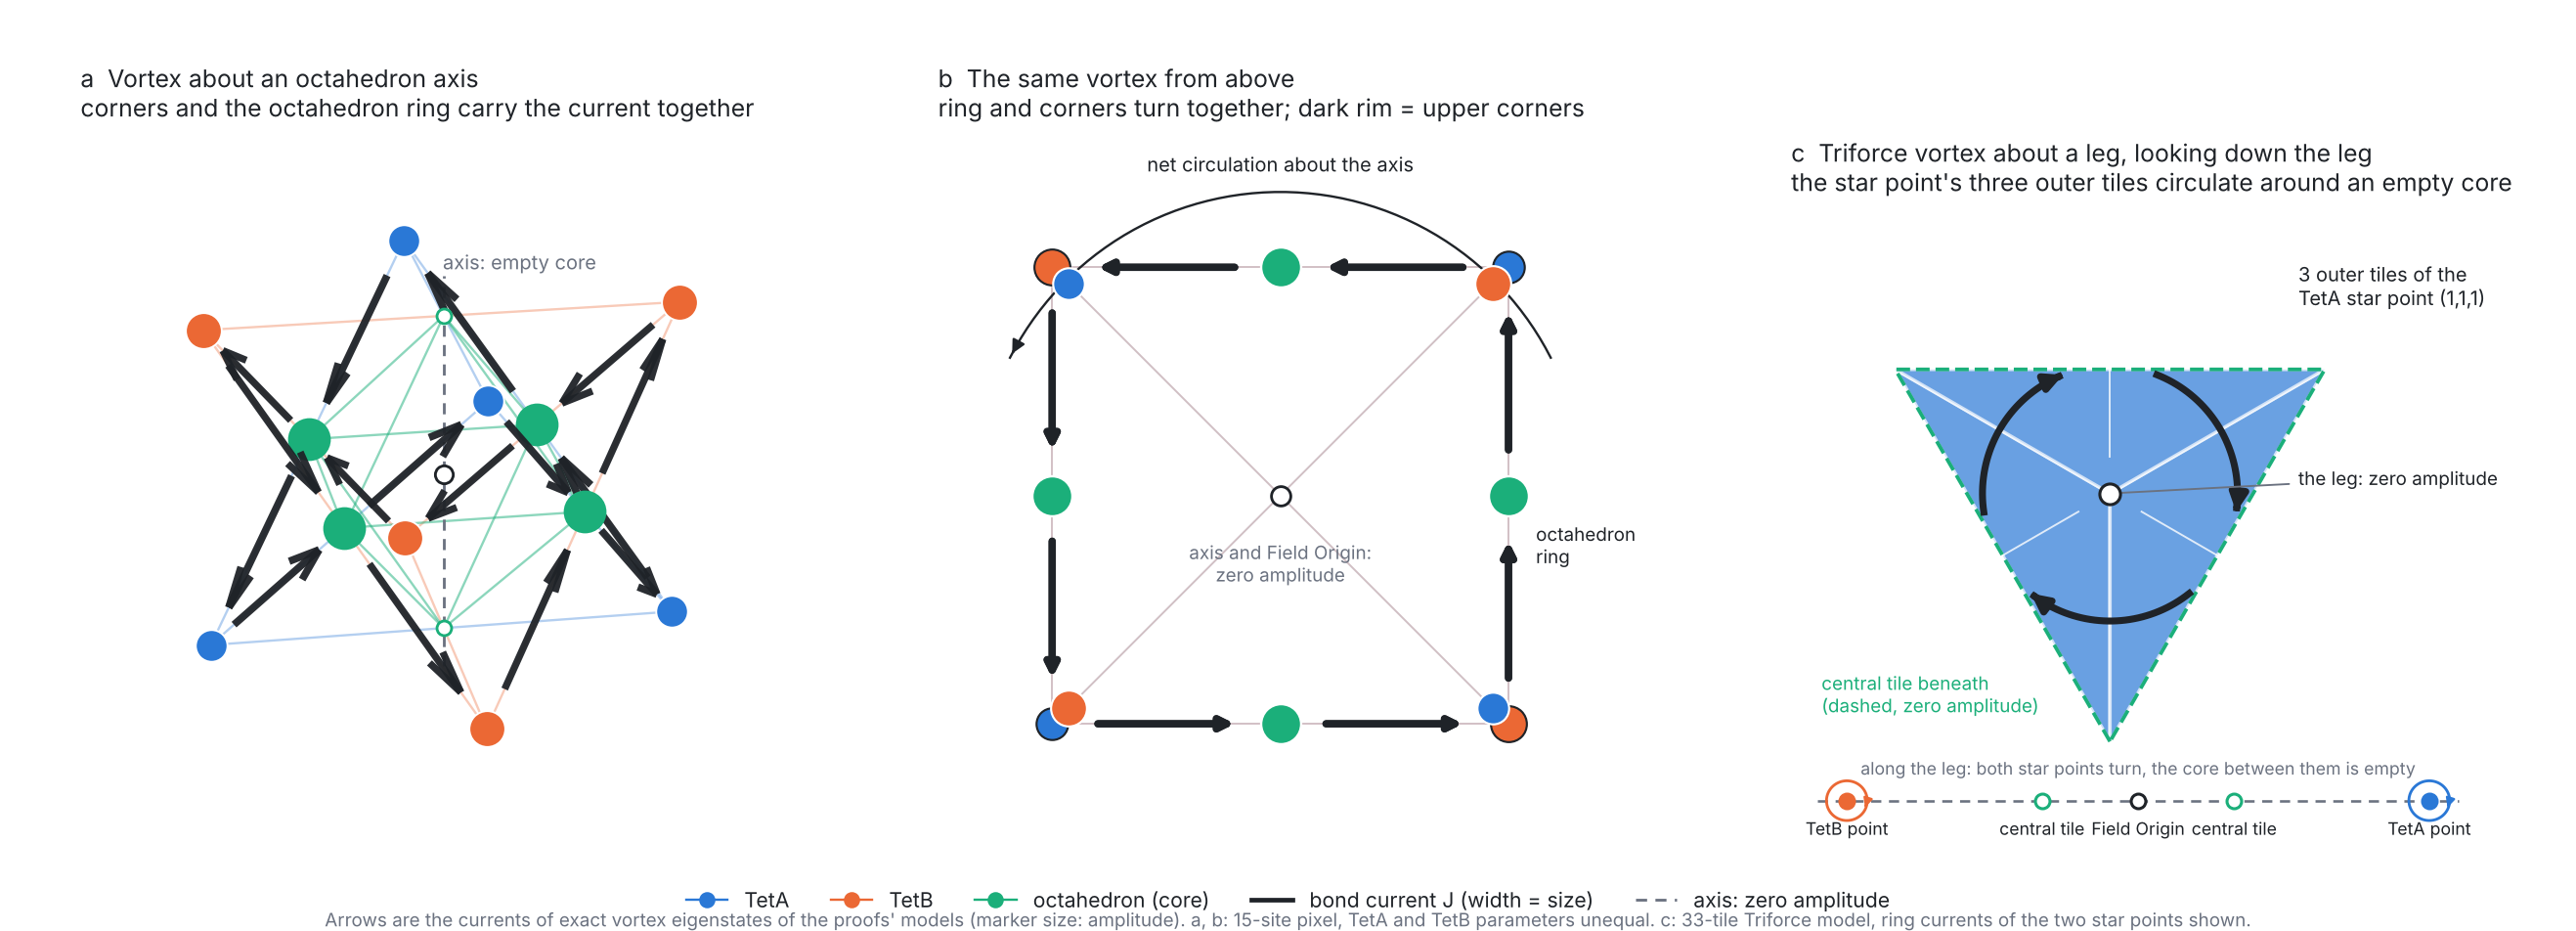
\includegraphics[width=\textwidth]{vortex_figure.png}
\caption{Bond currents $J_{i\to j}$ of exact vortex eigenstates (arrow
width: size; marker size: amplitude). (a) A vortex of the cube graph
$\mathcal C$ about an octahedron axis, with TetA and TetB parameters
unequal: the corners and the Field Origin's equatorial ring carry the
current together, and the axis carries zero amplitude (Lemma~2,
Theorem~\ref{thm:cube}). (b) The same state from above. (c) A
Triforce vortex on the cube's faces ($\mathcal T$), looking down a leg: the star
point's three outer tiles, its outer sub-channel, circulate around
the empty leg (Theorem~\ref{thm:triforce}).}
\label{fig:currents}
\end{figure*}

\begin{figure*}[h]
\centering
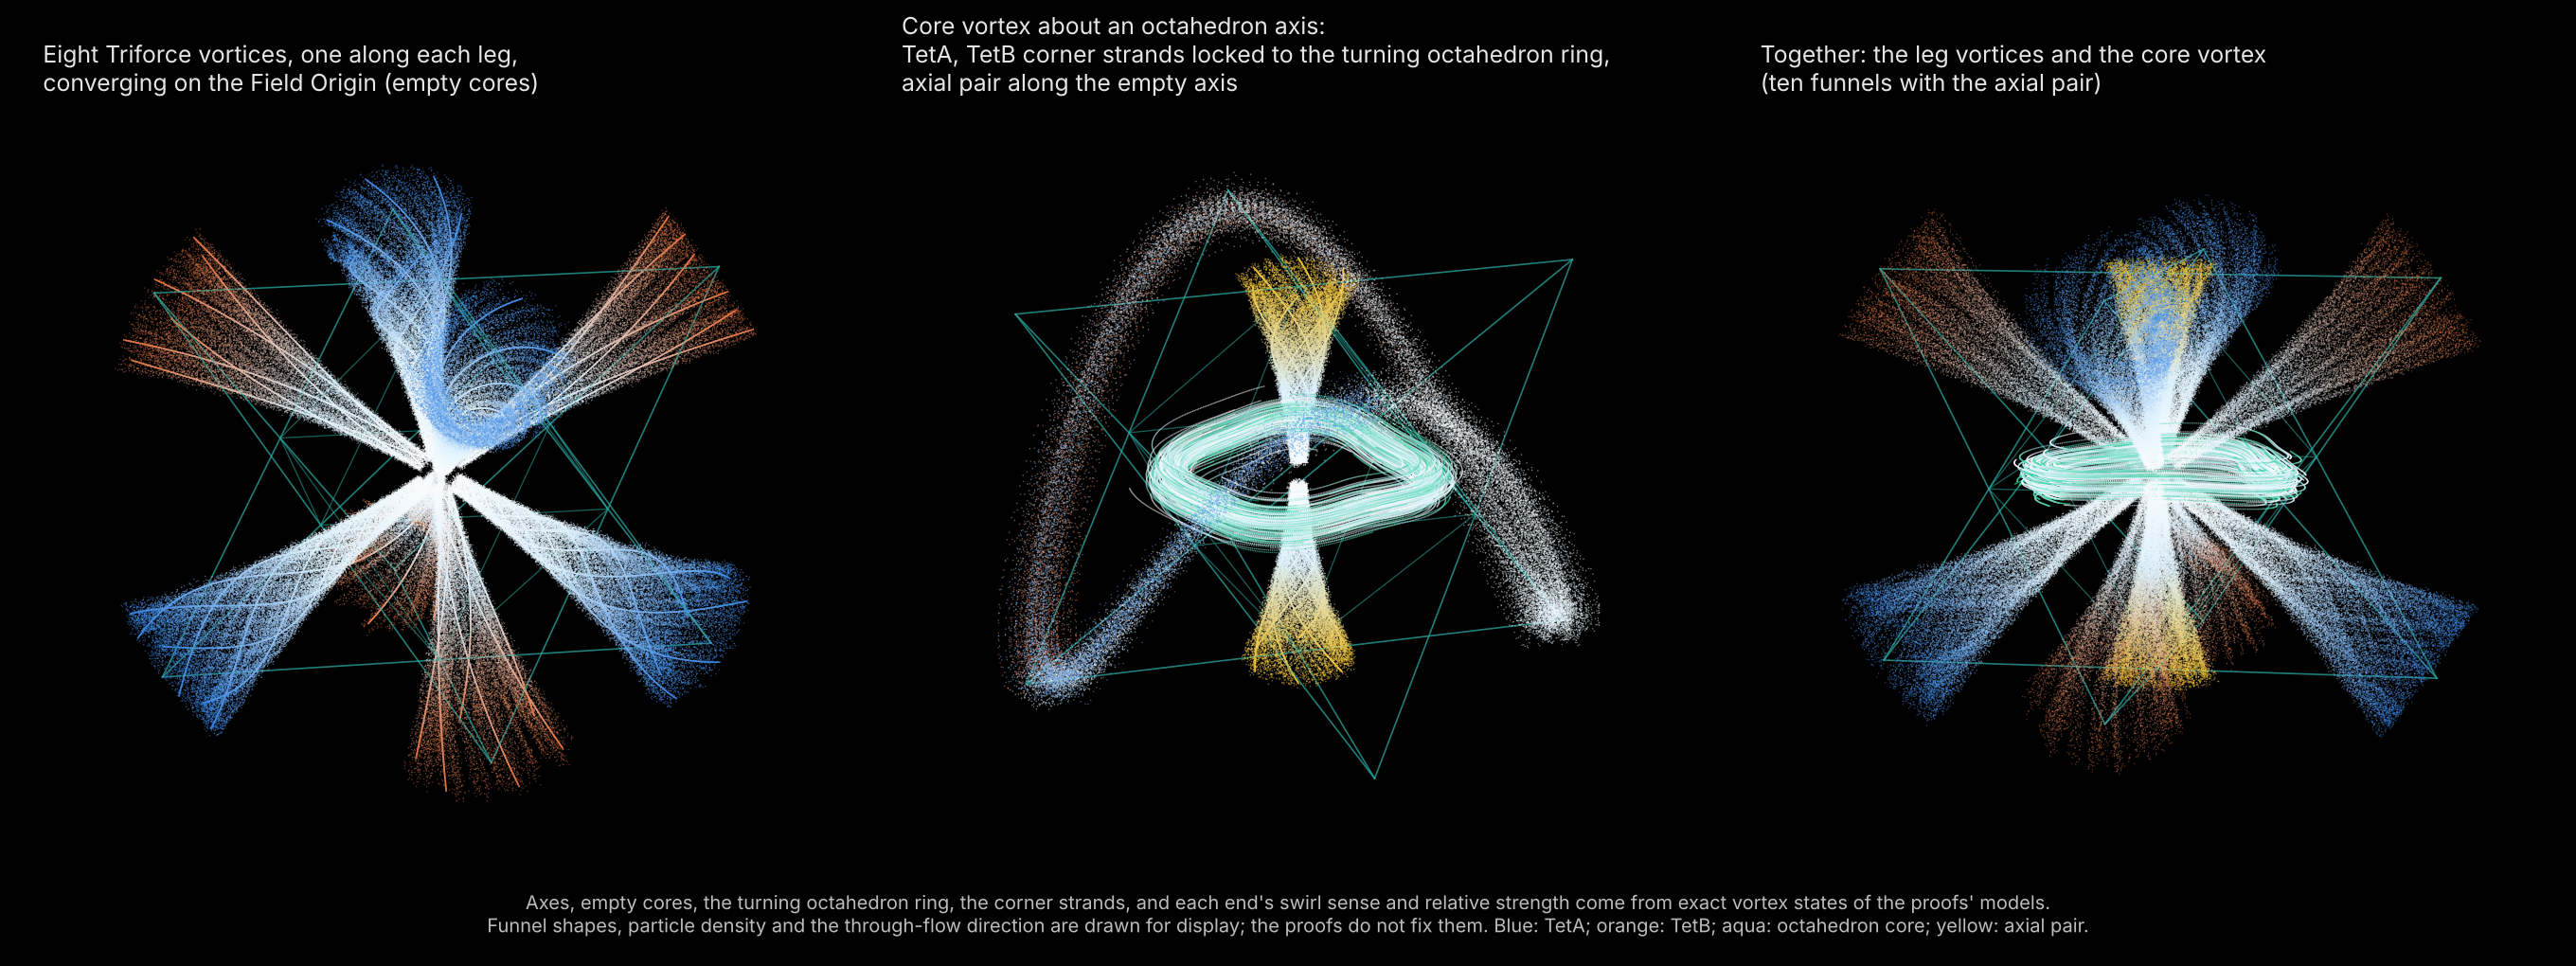
\includegraphics[width=\textwidth]{vortex_render.png}
\caption{Particle render of the vortices. Left: the eight leg
(Triforce) vortices. Centre: the core vortex about an octahedron
axis, with the Field Origin's turning equatorial ring (aqua), the TetA and TetB
corner strands locked to it, and the empty axis. Right: both together.
The axes, the empty cores, the turning ring, the corner strands and
each end's swirl sense and relative strength come from exact vortex
states of the models. The funnel shapes, particle density and the
direction of flow along an axis are drawn for display only; the
theorems do not fix them.}
\label{fig:render}
\end{figure*}

% ======================================================================

\section{Remarks}

\begin{remark}[Positioning]
That a real Hamiltonian with a cyclic symmetry has winding eigenstates
that carry ring currents is standard (see the remark \emph{Time reversal}, Section~1). What is specific here
is the structure on these graphs: the closed-form block and current of
the cube graph, the locking of the corners to the Field Origin's ring, the
interlacing and the explicit exceptional set, and the exact
$W \oplus W'$ structure of the Triforce with $W$ in closed form.
The standing waves are standard too: the Walsh--Hadamard functions are
the eigenmodes of the Boolean cube, the eigenvectors of its Laplacian
with eigenvalue $2\lvert S\rvert$~\cite{ODonnell2014}, and, read as
modes of coupled oscillators, each is a real standing wave that carries
no current. A nondegenerate eigenmode of a real $H$ is real up to a
phase, so circulation needs degenerate modes combined with complex
phases; here the degeneracy comes from the symmetries $S$ and $C$, of
order 4 and 3.
\end{remark}

\begin{remark}[Other bonds]
Adding the cube's edges gives the block (\ref{eq:block}) a TetA--TetB
entry and changes the secular equation; vortices still exist at random
parameter points, but Theorem~\ref{thm:cube} is not claimed for that
graph, and the corollary fails.
\end{remark}

\begin{remark}[GFD reading]
The following is interpretation, not part of the theorems. GFD
describes the Field Origin as the octahedral core where angular momentum
transfers, and as the eye of a self-sustaining vortex~\cite{NelsonColes}.
On the cube's points the circulation runs through the Field Origin, around its
equator, with its centre empty, and the eight corners turn with it, as a
flywheel locked to the ring. About a leg, the star point's outer
sub-channel (spatial coupling) turns around a core that is exactly the
gravitational coupling line, through the central tiles and the Field
Origin to the opposite star point~\cite{NelsonTriforce}. The theorems fix
the swirl, not any flow along the axis, which in the hourglass picture
of GFD is the through-flow at the throat~\cite{NelsonHourglass}. GFD takes TetA and TetB to
differ away from its transition $g/a_0 = 1$. If all TetA and TetB
parameters are equal, a plain quarter turn about an octahedron axis
becomes a symmetry, and Theorem~\ref{thm:cube}'s hypothesis
$\epsilon_A \neq \epsilon_B$ fails.
\end{remark}

\begin{remark}[Not claimed]
That the GFD field occupies these states, that these models are its
dynamics (the theorems concern the stated class), or any braiding. The
models are linear, while GFD's Field Origin is nonlinear, non-analytic
at zero field~\cite{NelsonColes}.
\end{remark}

\begin{remark}[History]
This proof supersedes an earlier research note that sampled the
Triforce model numerically and stated that every winding eigenstate
circulates; that holds on $W'$, not on all of $W$. The first version
of this proof counted currents with the reversed sign and omitted the
octahedron's edges; see the referee review in the same folder.
\end{remark}

% ======================================================================

\section*{Verification}

\texttt{verify\_vortices\_stellated\_octahedron.py} runs 81 checks.
Part~I (54) is exact arithmetic in $\mathbb Q(i)$ and $\mathbb Q(\omega)$
with Python fractions and no computer algebra: the geometry, $T_d$, the
Hamiltonians, the winding spaces, the empty axis, current conservation
across three half-planes, squarefreeness, nonzero current and ring
weight, antivortices, and the split $W\oplus W'$, at three fixed
pseudo-random rational points per model. Part~II (27) uses sympy, in
all parameters: the current convention, the block (\ref{eq:block}),
(\ref{eq:secular}), the interlacing, (\ref{eq:current}) for three
half-planes, Corollary~1 and its dependence on the bond set,
Proposition~\ref{prop:standing}, and Theorem~\ref{thm:triforce}(ii)--(iv),
including the representation-theoretic decomposition and the closed
form (\ref{eq:M}).

\begin{thebibliography}{99}

\bibitem{NelsonColes}
S.~Nelson,
\textit{GFD Coles Notes}, Field Dynamics Research (2026),
\url{GFD_COLES_NOTES.md}.

\bibitem{NelsonCoupling}
S.~Nelson,
\textit{The Coupling Algebra}, research note, Field Dynamics Research
(2026), \url{research/coupling-algebra}.

\bibitem{NelsonTriforce}
S.~Nelson,
\textit{Enterprise Triforce Synthesis}, Field Dynamics Research (2026),
\url{research/faces}.

\bibitem{NelsonHourglass}
S.~Nelson,
\textit{TetA and TetB as One Vortex}, research note, Field Dynamics
Research (2026), \url{research/vortex-hourglass}.

\bibitem{NelsonGram}
S.~Nelson,
\textit{The Gram Matrix of the Tetrad Equation},
Field Dynamics Research (2026),
\url{proofs/gram-matrix-tetrad-equation}.

\bibitem{Coxeter1973}
H.~S.~M.~Coxeter,
\textit{Regular Polytopes},
3rd ed.\ (Dover, New York, 1973).

\bibitem{London1937}
F.~London,
J.\ Phys.\ Radium \textbf{8}, 397 (1937).

\bibitem{Pople1956}
J.~A.~Pople,
J.\ Chem.\ Phys.\ \textbf{24}, 1111 (1956).

\bibitem{SteinerFowler2001}
E.~Steiner and P.~W.~Fowler,
J.\ Phys.\ Chem.\ A \textbf{105}, 9553 (2001).

\bibitem{BIL1983}
M.~B\"uttiker, Y.~Imry and R.~Landauer,
Phys.\ Lett.\ A \textbf{96}, 365 (1983).

\bibitem{ODonnell2014}
R.~O'Donnell,
\textit{Analysis of Boolean Functions}
(Cambridge University Press, Cambridge, 2014).

\bibitem{Serre1977}
J.-P.~Serre,
\textit{Linear Representations of Finite Groups}
(Springer, New York, 1977).

\bibitem{CLO}
D.~A.~Cox, J.~Little and D.~O'Shea,
\textit{Ideals, Varieties, and Algorithms},
4th ed.\ (Springer, Cham, 2015), ch.~3 (resultants).

\end{thebibliography}

\end{document}
